
\chapter{Experiments}\label{ch:experiments}

Based on the~\nameref{ch:data}, the~\nameref{ch:model} and the~\nameref{ch:optimization} we conducted various experiments,
and the evaluation of the selected models on the \textit{Clarin-dev} dataset are presented in this chapter.
The optimization of all models is uniform and presented in detail in the Chapter~\nameref{sec:model-optimization}.
We use the data augmentation with the following parameters $T=<5, 15>$, $T_{ratio}=0.3$, $T_{space}=10$, $F=20$, $m_f=1$,
which brings the most benefits, and they are the most accurate to the characteristics of
the Polish language (\ref{sec:data-augmentation})~\cite{igras2013}.
The decoding process is also uniform for all experiments, where
we use the beam of size 1024, and we do not use any external language model.


\section{Base Model}\label{sec:base-model}

We have to perform many experiments to adapt the basic model architecture
to the task conditions.
There are no studies on how deep neural networks \textit{end-to-end} manage to overcome
either the inflected language complexity or the highly limited training dataset.
The well-explored basic model is a reliable reference point for verification,
whether the presented \textit{Synthetic~Boosted~Model} is an attractive approach.
These series of experiments aim to verify the key components of the \acrshort{asr} model, which are
the \textit{Temporal~Convolution}, the \textit{Stacked~Recurrent~Layers} or the \textit{Time-Frequency~Convolution}.
The training corpus is for each experiment the same, and contains the \textit{Jurisdic}
as well as the \textit{Clarin-train} dataset (Chapter~\nameref{ch:data}).

\subsection*{Temporal Convolution}

The architecture of the first model is based on the \textit{Deep Speech} model, which is composed of five layers~\cite{hannun2014}.
The first layer is a one-dimensional, in the time domain, the \textit{Temporal Convolution} layer with
the filter size~15x80, and the number of filters equals to the width of the next layer.
Then there are two \textit{fully-connected} layers.
Both the convolution layer and the \textit{fully-connected} layers have the activation function
\textit{clipped rectified-linear} with a boundary value of~20.\footnote{
The activation function is limited in order to avoid the gradient exploding.}
The fourth layer is a bidirectional recurrent layer\texttt{LSTM}.
At the end of the model, there is a linear layer with the \textit{softmax} activation function.
At the time of training, the \textit{droupout} method~\cite{srivastava2014} is applied between
the \textit{fully connected} layers to reduce the effect of \textit{overfitting} (rate 10\%).

\begin{table}[h!]
\vspace*{10pt}
\centering
 \begin{tabular}{c c c c c}
  \toprule
  WER & CER & CTC Loss & Units & Model Size (M) \\
  \midrule
    34.87 &	7.09 &	10.23	& 650   & 8	 \\
    33.13 &	6.74 &	9.55	& 900   & 16 \\
    33.85 &	6.90 &	9.85	& 1300  & 32 \\
    33.85 &	6.89 &	10.01	& 1850  & 64 \\
  \bottomrule
 \end{tabular}
\caption{
The results of the \textit{Temporal~Convolution} models in terms of the number of parameters.
}
\label{table:temporal-convolution}
\end{table}

The table~\ref{table:temporal-convolution} presents the results of the four models that
have parameters between 8 and 64 million.
To compare the models, we use the \textit{Word Error Rate} metric (WER), but also
we report the \textit{Char Error Rate} (CER) metric, and the objective function values \textit{CTC Loss}.
The size of the model is exclusively modified by changing the width of all layers equally.


\subsection*{Stacked Recurrent Layers}

In this section, we present how \textit{stacked~recurrent} layers impact to the model performance.
Similar to the \textit{Deep Speech} model, the first layer is the \textit{Temporal Convolution} layer with
a filter dimension~15x80, and the number of filters equals to the width of the next layer.
Then there are bidirectional \acrshort{lstm} recurrent layers.
At the end of the model, there is a linear layer with an activation function \textit{softmax}.

\begin{table}[h!]
\vspace*{10pt}
\centering
 \begin{tabular}{c c c c c c}
  \toprule
   WER & CER & CTC Loss & LSTM size	& Architecture & Units (M)\\
   \midrule
    33.39	& 6.50	& 8.76  & 900 & 5-layers, 1 RNN & 16 \\
  \midrule
    29,05 &	5,82 & 7,79 & 550 &	5-layers & 16 \\
    24,06 &	4,78 & 6,49 & 800 &	5-layers & 32 \\
    20,73 &	4,27 & 5,73 & 650 &	7-layers & 32 \\
  \bottomrule
 \end{tabular}
\caption{
The architectures composed of the stack of recurrent layers.
}
\label{table:stacked-recurrent-layers}
\end{table}

The table~\ref{table:stacked-recurrent-layers} shows the experiment results.
Furthermore, our attempts to do the \textit{Batch Normalization} in the \acrshort{lstm} layer
before each activation function do not bring positive results~\cite{amodei2015}.
Unfortunately, the effective implementation \textit{CuDNN-LSTM}, presented in the Chapter~\ref{sec:system-optimization},
precludes to implement the \textit{sequence-wise} normalization~\cite{laurent2015}, which in consequence, is not explored.


\subsection*{Time-Frequency Convolution}

In this section, we present how the \textit{Time-Frequency Convolution} layer impacts model performance.
At the beginning of the model, there is a two-dimensional \textit{convolution Layer}.
Then there are 5 bidirectional recurrent \acrshort{lstm} layers with the width of~650.
At the end of the model, there is a linear layer with the \textit{softmax} activation function.
In the two-dimensional convolution layers shown here, the first dimension is time and
the second dimension is frequency.
The width of the filter in the time domain is constant and equals~15.

\begin{table}[h!]
\vspace*{10pt}
\centering
 \begin{tabular}{c c c c c c c}
  \toprule
    WER & CER & CTC Loss & Type	& Channels	& Filter dimension	& Stride \\
   \midrule
    20,73 & 4,27 & 5,73	& 1-layer 1D & 650	        & 15	        & 1x1       \\
  \midrule
    16,60 & 3,39 & 4,80	& 1-layer 2D & 32	        & 15x41	        & 2x2       \\
    22,35 & 4,75 & 6,86	& 2-layer 2D & 32, 64	    & 15x41, 15x21	& 2x2, 2x1  \\
  \bottomrule
 \end{tabular}
\caption{
The impact of the \textit{Time-Frequency~Convolution} layers.
}
\label{table:time-frequency-convolution}
\end{table}

The results are presented in the table~\ref{table:time-frequency-convolution}
The \textit{stride} (a step of convolution operation) is applied
both in the frequency as well as in the time domain.
The length of the sequence to be processed by subsequent recurrent layers is halved,
which reduces the duration of the experiments almost two times.


\section{Synthetic Boosted Model}\label{sec:synthetic-boosted-model}

In this section, we introduce two experiment series that presents
the use of the \textit{Synthetic~Boosted Model} on different training datasets.
In the \textit{Entire Dataset} section, we perform experiments on the entire training dataset,
which is composed of the \textit{Jurisdic}, the \textit{Clarin-train}, and synthetic data.
Afterward, in the \textit{Limited Dataset} section, the training corpus is strongly reduced,
and only consists of the \textit{Clarin-train} and synthetic data.


\subsection*{Entire Dataset}

The \textit{Synthetic~Boosted~Model} is composed of two integrated parts, the \textit{Phoneme~Model}
and the \textit{Synthetic~Language~Model}, therefore, training is divided into two stages (Chapter~\nameref{ch:model}).
Initially, we train the \textit{Phoneme~Model} (model named \textit{Phoneme} in the table~\ref{table:entire-dataset})
on the training dataset composed of the \textit{Jurisdic}, the \textit{Clarin-train} and an additional
300~hours of synthetic data.
The model contains 7 hidden layers.
The first layer is the two-dimensional \textit{Convolutional Layer}, where the receptive field size
is~15x41 (time-frequency), and the number of channels equals~32.
Then, there are 5~bidirectional recurrent \acrshort{lstm} layers with the width of~650.
At the end of the model, there is a linear layer with an activation function \textit{softmax},
which is deleted after the training.
The objective function is the weighted sum of the \textit{CTC~Loss} and the \textit{Adversarial~Loss} (theirs weights are equal).
The \textit{Adversarial~Loss} evaluates the hidden states of the last \acrshort{lstm} layer.\footnote{
We have done experiments, where the \textit{Adversarial~Loss} evaluates either the first or the third \acrshort{lstm} representations.
However, the training is stopped on the high \textit{plateau} due to the strong regularization.
}

\begin{table}[h!]
\vspace*{10pt}
\centering
 \begin{tabular}{c c c c c l}
  \toprule
    WER	    & CER	 & CTC Loss	 & Auth.~Audio	&  Syn.~Audio	& Model         \\
    \midrule
    16,60	& 3,39	& 4,80	    & 385		    &               & Base          \\
    15,21	& 3,12	& 4,25	    & 385	        & 300	        & Phoneme       \\
    14,33	& 2,78	& 3,99	    & 385	        & 1000	        & Boosted       \\
  \bottomrule
 \end{tabular}
\caption{
The results of the \textit{Synthetic~Language~Model} where the training dataset is composed of
the \textit{Jurisdic}, the \textit{Clarin-train} and an additional 1,000 hours of synthetic data.
}
\label{table:entire-dataset}
\end{table}

The second stage is to train the \textit{Synthetic~Language~Model} on the training dataset composed of
the \textit{Jurisdic}, the \textit{Clarin-train} and an additional 1000 hours of synthetic data
(model named \textit{Boosted} in the table~\ref{table:entire-dataset}).
The \textit{Phoneme~Model} is frozen (weights are not updated), therefore, it plays exclusively
a feature extractor role at this stage.
It provides input data (hidden states $h$ of the last layer \acrshort{lstm}) for the \textit{Synthetic~Language~Model}.
The \textit{Synthetic~Language~Model} contains 5 hidden layers.
The first layer is the \textit{projection} layer, a narrow \textit{fully-connected} layer,
with the width of~36, and the activation function \textit{clipped rectified-linear} with the boundary value of~20.
Then there are 3~bidirectional recurrent \acrshort{lstm} layers with the width of~650.
At the end of the model, there is a linear layer with the activation function \textit{softmax}.

\subsection*{Limited Dataset}

In these experiments, the authentic training dataset is strongly reduced, where
the training corpus solely consists of the \textit{Clarin-train} and synthetic data.
Both the \textit{Phoneme~Model} and the \textit{Synthetic~Language~Model}, as well as the training policy,
are the same as those presented in the subsection \textit{Entire Dataset}.
We do series of experiments in which we try to customize the \textit{Phoneme Model}
to the limited dataset.
In fact, the adjustments do not bring noticeable improvements.

\begin{table}[h!]
\vspace*{10pt}
\centering
 \begin{tabular}{c c c c c l}
  \toprule
    WER	    & CER	 & CTC Loss	 & Auth.~Audio	  &  Syn.~Audio	    & Model                 \\
    \midrule
    21,69	& 4,22	 & 5,71	     & 34		      &                 & Base                  \\
    21,37	& 4,20	 & 5,92	     & 34		      &                 & Base+                 \\
    21,13	& 4,20	 & 5,66	     & 34	          &  34	            & Phoneme               \\
    19,81	& 3,96	 & 5,67	     & 34	          &  1000	        & Boosted               \\
    \midrule
    16,60	& 3,39	 & 4,80	     & 385            &                 & Base                  \\
  \bottomrule
 \end{tabular}
\caption{
The results of the \textit{Synthetic~Language~Model} where the training dataset is composed of
the \textit{Clarin-train} and an additional~1000 hours of synthetic data.
}
\label{table:limited-dataset}
\end{table}

The results are presented in the table~\ref{table:limited-dataset}.
To the comparison, we present the \textit{Base+} model, which has the same architecture as the \textit{Boosted} model
(and use the frozen \textit{Base} model), but it is trained exclusively on the \textit{Clarin-train} dataset.


\section{Conclusions}\label{sec:conclusions}

\subsection*{Base Model}

We began our experiments with the model architecture based on the \textit{Deep~Speech} model.
The model with 16 million parameters achieves the best result, where the WER equals 33.13\%.
The number of model parameters strongly depends on the size of the training dataset.
Our dataset is much smaller than the one presented in~\cite{hannun2014},
therefore, we achieve similar results, even when we reduce the number of parameters eight times
beside the \textit{Deep~Speech} model.
The table~\ref{table:samples-baseline} shows the selected examples of model predictions.
Despite the high WER level, it is apparent that the model has learned different spelling rules,
for instance \emph{zdążyłem}, \emph{żadnej}, and \emph{alkoholiku}.
However, the WER score above 30\% is too high to make the system useful.

\begin{table}[h!]
\vspace*{10pt}
\small
\centering
 \begin{tabular}{p{5cm} | p{5cm}}
  \toprule
  Model prediction & Correct transcription \\
  \midrule
  ja nie zdążyłem rozpocząć żadnej działalności a\textbf{l}i & ja nie zdążyłem rozpocząć żadnej działalności a\textbf{n}i               \\[5pt]
  słowami takimi jak brydziarzu złodzieju alkoholiku & słowami takimi jak bry\textbf{n}dziarzu złodzieju alkoholiku                     \\[5pt]
  dowodowymi i \textbf{określe\,nia} wartości poszczególnych dowodu & dowodowymi i \textbf{określenia} wartości poszczególnych dowodów  \\
  \bottomrule
 \end{tabular}
\caption{The selected predictions of the \textit{Temporal~Convolution} model with the layer width~900 (16~million parameters).}
\label{table:samples-baseline}
\end{table}

In the \textit{Temporal~Convolution} models, the first three layers build a representation solely on a small context of a signal.
The broader context, done by replacing \empth{fully~connected} layers to recurrent layers, brings better performance, what
we presented in the \textit{Stacked~Recurrent~Layers} experiments.
The best model architecture has 32 million parameters and consists of 7 layers,
including 5 \texttt{LSTM} layers with the width of 650.
Although the model is composed of 7 layers (a gradient propagation travels a long way),
the model optimization is stable thanks to the data augmentation technique,
the large batch size (256), and uniform sample lengths from 3 to 7 words (Chapter~\nameref{ch:data}).
We are aware that by doing so, we lose the ability to represent contexts longer than 7 words.

In \textit{Time-Frequency~Convolution} experiments, we present that the use of a single
two-dimensional convolutional layer significantly improves model generalization (the WER score drops to 16.60\%).
The one-dimensional (time) convolutional layer has a large perception area (15x80)
and is non-resistant to shifts in the frequency domain.
We analyze the filters of the one-dimensional convolutional layer,
which shows that most of the filters are unused.
The used filters are grouped into several types (similar shapes), and they are concentrated in tiny areas.
A two-dimensional convolutional layer accurately resolves these issues.
It groups filters of the similar shape (the number of \textit{channels} is reduced), which are shifted in the frequency domain.



\subsection*{Synthetic Boosted Models}

The experiments presented in the section~\ref{sec:synthetic-boosted-model} confirms
that the large synthetic dataset can be successfully used in \textit{end-to-end} speech recognition models.
The \textit{Synthetic~Boosted~Model} trained on the entire synthetically augmented
dataset achieves more than 13\% absolute better the WER score, which equals 14,33\%.

In the figure~\ref{fig:synthetic-lm-improvements}, we present two matrices.
On the left is the matrix grouping mistakes of the \textit{Synthetic~Boosted~Model}
by the \textit{Char~Edit~Distance} and the \textit{Word~Edit~Distance}.
We can see that more than 800 samples have a single spelling mistake.
The most difficult to correct mistakes are on the out of a diagonal, which have
high values of the \textit{Char~Edit~Distance}.
On the right side, we see the corrected mistakes
with respect to the \textit{Phoneme~Model}.
We can observe that the \textit{Synthetic~Language~Model} also corrects mistakes
that have the high \textit{Char~Edit~Distance} value.

\begin{figure}[h]
    \centering
    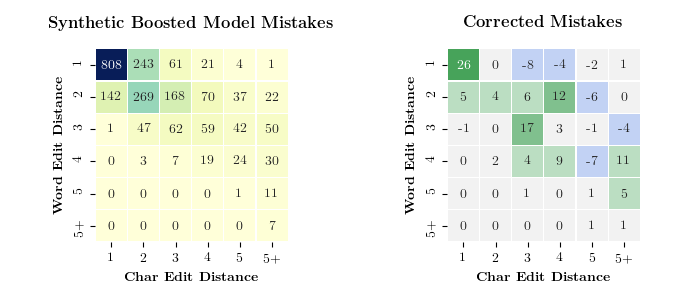
\includegraphics[width=1\textwidth]{figures/experiments-synthetic-lm-improvements.png}
    \caption{
On the left, the grouped mistakes of the \textit{Synthetic~Boosted~Model} by
the \textit{Char~Edit~Distance} and the \textit{Word~Edit~Distance}.
On the right, the corrected mistakes, which are defined as the difference between
the \textit{Phoneme~Model} and the \textit{Synthetic~Boosted~Model}.
}
    \label{fig:synthetic-lm-improvements}
\end{figure}

The \textit{Synthetic~Boosted~Model} trained on the \textit{Limited~Dataset} also outperforms the \textit{Base Model}
with almost 10\% absolute better WER score, which equals 19.81\%.
The difference in the performance of two \textit{base~models},
which are trained on 34 and 385 hours of authentic data, equals 5.09 of WER score.
The \textit{Synthetic~Boosted~Model} covers 36.94\% of this difference using 1000 hours of synthetic data.
We are aware that there could be many factors which cause the inefficient use of synthetic data.
Nonetheless, we introduce further one of them.

\begin{figure}[h]
    \centering
    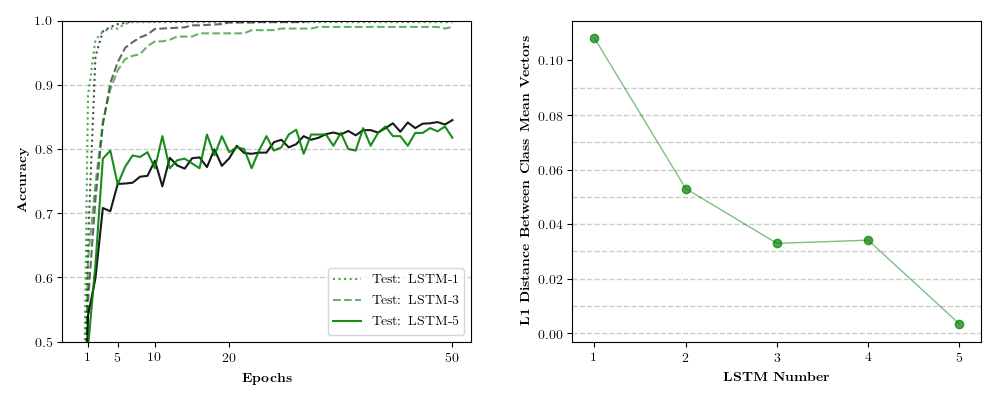
\includegraphics[width=0.9\textwidth]{figures/experiments-representation-disambiguation.png}
    \caption{
The linear separability test of the representations $h$ returned by the~\textit{Phoneme~Model}.
Classifiers try to predict whether the representations $h$ comes from authentic or synthetic data.
}
    \label{fig:representation-disambiguation}
\end{figure}

We do a test to check the linear separability of the representation $h$ returned by the \textit{Phoneme~Model}.
From the training corpus, we selected a thousand samples of authentic and synthetic data~(the~ratio~1~to~1).
Then, we process these samples using the~\textit{Phoneme~Model}, in a purpose to
collect the hidden states $h$ for each \acrshort{lstm} layer.
Finally, we build a set of simple binary classifiers, which try to predict whether the representation  $h$
comes from authentic or synthetic data (different classifier for each layer).\footnote{
The classifiers are the same, and they are composed of one neuron with the activation function \textit{sigmoid}.
}

The classifier that analyzes the activation of the first \acrshort{lstm} layer, immediately
and error-free recognizes the activation source (figure~\ref{fig:representation-disambiguation}).
In accordance with our expectations, subsequent classifiers have larger
difficulties in identifying the data source.
On the right-hand side, the graph presents the values of the \textit{Adversarial~Loss}
depending on the depth of the \acrshort{lstm} layer.
We can see that despite the near-zero loss function value (the fifth layer), the linear classifier
separates with the high precision the activations from authentic and synthetic
data (the \textit{accuracy} over 80\%).
The further investigation of the other \textit{Adversarial~Loss} function is highly recommended.
